%%%%%%%%%%%%%%%%%%%%%%%%%%%%%%%%%%%%%%%%%%%%%%%%%%%%%%%%%%%%%%%%%%%%%%%%%%%%
\documentclass[a4j,11pt]{article}
\usepackage{latexsym}
\usepackage{cite}
\usepackage[dvips]{graphicx}
\usepackage{amsfonts}
\usepackage{amsmath}
%\usepackage{amsthm}
\usepackage{amssymb}
\usepackage{marvosym}
\usepackage{pifont}
\usepackage{ascmac}
\usepackage{url}
\usepackage{booktabs}
\usepackage{float}
\usepackage{bm}
\usepackage{cite}
\usepackage{arydshln}
\usepackage{comment}
\usepackage[algo2e,ruled]{algorithm2e}
\usepackage{stackengine} % for addstackgap

% \setlength{\oddsidemargin}{1.0cm}
% \setlength{\evensidemargin}{1.0cm}
\renewcommand{\floatpagefraction}{0.7}
\renewcommand{\baselinestretch}{1.3}
\renewcommand{\arraystretch}{0.8}
\pagestyle{empty}

\newcommand{\tss}{\mathrm{TSS}}
\newcommand{\mse}{\mathrm{MSE}}
\newcommand{\mysum}[1]{\sum_{i \in[#1]}}
\newcommand{\mymin}[1]{\min_{\scalebox{1.0}{$#1$}}}
\newcommand{\mymax}[1]{\max_{\scalebox{1.0}{$#1$}}}
\newcommand{\myargmin}[1]{\min_{\scalebox{1.0}{$#1$}}}
\newcommand{\argmax}{\mathop{\rm arg~max}\limits}

\newcommand{\Graph}{\mathcal{G}} % Graph Space
\newcommand{\Gs}[1]{\mathcal{G}_{\scalebox{0.9}{$#1$}}} % with subscript
\newcommand{\Y}{\mathcal{Y}} % response label Y Space
\newcommand{\D}{\mathcal{D}} % Data
\newcommand{\I}{\mathbb{I}} % indicator function
\renewcommand{\S}{\mathcal{S}} % subgraph Space
\renewcommand{\H}{\mathcal{H}} % hypothesis space
\renewcommand{\labelenumi}{\arabic{enumi})}
\renewcommand{\a}{\bar{a}}
\renewcommand{\b}{\bar{b}}


%% thick hline
\makeatletter
\def\thickhline{%
  \noalign{\ifnum0=`}\fi\hrule \@height \thickarrayrulewidth \futurelet
   \reserved@a\@xthickhline}
\def\@xthickhline{\ifx\reserved@a\thickhline
               \vskip\doublerulesep
               \vskip-\thickarrayrulewidth
             \fi
      \ifnum0=`{\fi}}
\makeatother

\newlength{\thickarrayrulewidth}
\setlength{\thickarrayrulewidth}{2\arrayrulewidth}

%% command set for circled graph notations
%\renewcommand{\v}[1]{\textcircled{\raisebox{-0.7pt}{\footnotesize{#1}}}}
\renewcommand{\v}[1]{\textcircled{\raisebox{-0.7pt}{\footnotesize{#1}}}}
\newcommand{\e}{\text{--}}

%% for linear nonlinear
\newcommand{\gxxx}[3]{\v{#1}\e\v{#2}\e\v{#3}}

%% for stackengine
\renewcommand{\ss}[2]{\addstackgap{\shortstack{#1\\#2}}}

%% for acc table
%\renewcommand{\*}[1]{\hspace{5pt}#1\raisebox{2pt}{\scriptsize *}}
\newcommand{\fst}[1]{{\bf #1}}
\newcommand{\fss}[2]{\addstackgap{\shortstack{\bf #1\\#2}}}


% for algorithm
\SetKwData{t}{tss}
\SetKwData{mt}{min\_tss}
\SetKwData{bg}{best\_$g$}
\SetKwData{g}{$g$}
\SetKwData{n}{n}
\SetKwData{bound}{bound}
\SetKwProg{Fn}{Function}{}{}
\SetKwComment{cmt}{$\triangleright$~}{}
\renewcommand*{\algorithmcfname}{Alg.}

% theorem
\newtheorem{definition}{Definition}
\newtheorem{theorem}{Theorem}
\newtheorem{proof}{Proof}
\def\qed{\hfill $\Box$}

\newcommand{\TODO}[1]{\textcolor{green!50!black}{{\footnotesize TODO }#1}}
\newcommand{\COMMENT}[1]{\textcolor{orange!80!black}{{\footnotesize Comment: }#1}}
\renewcommand{\TODO}[1]{} \renewcommand{\COMMENT}[1]{} % switch TODO COMMENT on off by comment out in
\newcommand{\SKIP}[1]{#1}
\renewcommand{\SKIP}[1]{} % switch SKIP on off by comment in out

%%%%%%%%%%%%%%%%%%%%%%%%%%%%%%%%%%%%%%%%%%%%%%%%%%%%%%%%%%%%%%%%%%%%%%%%%%%%

\begin{document}
\begin{titlepage}
 \setcounter{page}{0}
  \begin{center}
   \vspace*{2.0cm}
   \LARGE
   Fast Search of Subgraphs Discriminative for Classification and Regression
   \\
   \vfill
   \LARGE
   Graduate school of Infomation Science and Technology, Hokkaido Universisy\\
   \vspace{2ex}
   %名前
   Ryo Shirakawa\\
   \vspace{2ex}
   %日付
   %(ex)2011年3月\\
   \vspace*{2cm}
  \end{center}
\end{titlepage}
\tableofcontents \thispagestyle{empty}
 \newpage
 \listoffigures

 \listoftables
 \clearpage 
 \pagestyle{plain} 
%\maketitle

%%%%%%%%%%%%%%%%%%%%%%%%%%%%%%%%%%%%%%%%%%%%%%%%%%%%%%%%%%%%%%%%%%%%%%%%%%%%

\begin{abstract}
Recently, in various fields such as computational chemistry and bioinformatics,
attention has been paid to classification and regression
of data whose inputs are graphs of arbitrary size and shape, 
sometimes called graph classification/regression.
In these problems,
whether a certain subgraph is included or not 
is a fundamental feature for graphs that have no direct descriptors available.
The simplest solution, 
enumerating subgraph patterns and use them as features, is so expensive 
since the number of possible subgraph patterns are intractably large 
due to the combinatorial explosion.
Currently, discriminative pattern mining has been studied and given a good solution to this problem.
The previous search method for such discriminative subgraph patterns 
tries to find the best one by the depth first search with some pruning rules.
Such a exact search, however, is costly for heavily repeated use, 
which is necessary to obtain the number of features enough for high performance classifiers or regressors.
To overcome this computational cost issue, 
we propose two approximate algorithms based on 
$(i)$ best first search, $(ii)$ Monte Carlo Tree Search(MCTS). 
We demonstrate effectiveness of our proposed methods by comparing performance 
in real problems using QSAR datasets.

\end{abstract}

\section{Introduction}
Graphs are fundamental data structures for representing combinatorial objects 
such as chemical compounds, networks and others.
However, precisely because of their combinatorial nature, 
it is usually difficult to understand the underlying trends in large datasets of graphs.
The rapid increase in data in recent years also includes data
represented as graphs, and thus supervised learning in which the inputs are graphs of
arbitrary size and shape has gained considerable attention
in the fields of computer vision \cite{Harchaoui:2007, Nowozin:2007, Barra:2013, Bai:2014a},
chemoinformatics \cite{Kashima:2003, Tsuda:2007,Saigo:2008a, Saigo:2009,Mahe:2009, 
Vishwanathan:2010, Shrvashidze:2011, Takigawa:2013, takigawa:2017},
bioinformatics\cite{Borgwardt:2005, Karklin:2005, Takigawa:2011b} 
and computational chemistry\cite{Kearnes2016, gilmer:2017} 
and natural language processing\cite{Kudo:2005}. 

Some of these problems have graph descriptors prepared in advance, 
such as molecular dataset\cite{james:2004, durant:2002}, 
but others have no direct descriptors available.
For these problems, the most fundamental features are subgraph indicators, 
i.e., if a subgraph is embedded in the given graph or not,
because many reactions and events are attributed to those substructures.
However, the number of all possible subgraph patterns is intractably large 
due to the combinatorial explosion, 
so that it is difficult to enumerate all subgraphs in a realistic time for a given dataset.
Therefore, it is necessary to restrict the subgraph candidate on the basis of some criterion.
Frequent subgraph mining \cite{Yan:2002, Nijssen:2004} is one method in this approach.
However, since it chooses subgraphs acording to the frequencies, 
it is possible to overlook the importance of subgraphs.
On the other hand, discriminative pattern mining techniques \cite{Fan:2008, Saigo:2009, Shirakawa:2018} 
choose subgraphs according to a model-based discriminative criteria, 
and these not likely to overlook important patterns for learning.
Because of these merits, the present paper also adopts this approach.

\subsection{Related Work}
%TODO
\label{sec:relatedwork}
Related works \cite{Saigo:2009, Shirakawa:2018} search the discriminative subgraph pattern
using depth first policy with branch and bound method.
While these methods perform efficient searches by designing tricky pruning, 
search policy of depth first is naive and 
they still suffer from computational costs for some domain or large datasets.

\subsection{Our Approach}
\label{sec:ourapproach}
To overcome the above difficulty, 
we propose the more efficient two algorithms
using Best First Search and Monte Carlo tree search (MCTS).
The efficiency of these building-block algorithms are already known in some domains, 
so that in this paper we apply them to our graph classification/regression problem.

\section{Preliminaries}
\subsection{Notations}
Let $[n]$ be a set of integers $\{1,2,\dots,n\}$ 
and let $\I(P)$ be the indicator of a predicate $P$, 
i.e., $\I(P)=1$ if $P$ is true, else $0$. 
A labeled graph is represented by a 4-tuple $G = (V, E, \mathcal{L}, l)$, 
where $V$ is a set of vertices, $E \subset V \times V$ is a set of undirected edges, 
$\mathcal{L}$ is a set of labels, and $l: V \cup E \rightarrow \mathcal{L}$ is a mapping 
that assigns a label to each vertex or edge.
We denote a subgraph isomorphism, i.e., if $g$ is a subgraph of $G$, as $G \sqsupseteq g$ 
and its negation as $G \not\sqsupseteq g$. 
Thus, a subgraph indicator $\I(G \sqsupseteq g) = 1$ if $G \sqsupseteq g$, otherwise 0.
We also denote the training set of pairs of input graph $G \in \Graph$ 
and its output responses $y \in \Y$ as
\begin{equation}
  \label{eq:train_data}
  \D = \{(G_1,y_1),(G_2,y_2),\dots,(G_N,y_N)\}.
\end{equation}
We assume that $\Graph$ is a set of all finite-size, connected, discretely-labeled, undirected graphs. 
We denote any set of graphs of size $N$ by $\Graph_N = \{G_i\mid i \in [N]\}$, 
and the set of all possible connected subgraphs 
as $\S_N = \bigcup_{G \in \Graph_N} \{g \mid G \sqsupseteq g\}$.

\begin{definition}{(subgraph isomorphism)}
	For two graphs, $G' = (V', E', \mathcal{L}', l')$ and $G = (V, E, \mathcal{L}, l)$, 
	$G'$ is subgraph isomorpic to $G$ iff there exist an injective mapping $\phi: V' \rightarrow V$, 
	s.t., (1) $\forall v \in V', l'(v) = l(\phi(v))$, 
	(2) $\forall (v_{1}, v_{2}) \in E', (\phi(v_{1}), \phi(v_{2})) \in E$ and
	(3) $l'(v_{1}, v_{2}) = l(\phi(v_{1}), \phi(v_{2}))$.
\end{definition}

\subsection{Search Space for Subgraphs}
\label{sec:subgraphMining}
In supervised learning from graphs, we represent each input graph $G_i \in
\Graph_N$ by the characteristic vector $(\I(G_i \sqsupseteq g) \mid g \in
\S) $ with a set $\S$ of relevant subgraph features. However, since $\S$ is not
explicitly available when the learning phase starts, we need to
simultaneously do searching and constructing of $\S$ during the learning process.
In order to define an efficient search space for $\S_N$, i.e., any subgraphs occurring in $\Graph_N$,
the techniques for \textit{frequent subgraph mining} \cite{Yan:2002, Nijssen:2004} are
useful. Note that any subgraph feature
$g \in \S_N$ can occur multiple times at multiple locations in a single graph,
even if $\I(G_i \sqsupseteq g) = 1$.

In the present paper, we use the search space of the gSpan algorithm \cite{Yan:2002},
which performs a depth-first search on the tree-shaped search spaces on $\S_N$,
referred to collectively as an \textit{DFS code tree}, as shown in Figure~\ref{fig:search_tree}.
Each node of the DFS code tree holds a subgraph feature $g'$ that
extends the subgraph feature $g$ at the parent node by one edge, namely, $ g' \sqsupseteq g $.

\begin{figure}[t]
  \centering
  \includegraphics[width=0.5\linewidth]{img/search_tree.eps}
  \caption{DFS code tree. Search space for subgraphs that appear in the training dataset.}
  \label{fig:search_tree}
\end{figure}

The following \textit{anti-monotone} property of
subgraph isomorphism over the DFS code tree on $\S_N$ can be used to
derive the efficient search-space pruning of the gSpan algorithm:
\begin{equation}
  \label{eq:propSubgraph}
  g' \sqsupseteq g, \quad 
  G_i \not \sqsupseteq g \Rightarrow G_i \not\sqsupseteq g'. % period
\end{equation}

\subsection{Discriminative Criterion}
\label{sec:criterion}
In the previous methods, the discriminating power are calculated 
by model-based criterioa or statistical criterioa such as information gain.
In present paper, the discriminating power ($Discriminative Score: DScore$) is defined 
by the following equation.
%\begin{eqnarray}
  %\label{eq:score_C}
  %CScore(g) = \max \Big[ \sum_{n=1}^{N} y_{n} (2\I(G_{n} \sqsupseteq g) - 1), \sum_{n=1}^{N} y_{n} (2\I(G_{n} \not\sqsupseteq g) -1) \Big]
%\end{eqnarray}
%This score is the sum of the values that take +1 if the graph label prediction is correct and -1 otherwise.
%When predicting the graph labels with real values, $RegressionScore$ $(RScore)$ is used defined as (\ref{eq:score_R}).
\begin{eqnarray}
  \label{eq:score_R}
  DScore(g) &=& \tss(\D_1(g)) + \tss(\D_0(g)) \\
  \tss(\D) &=& \sum_{i \in [N]}
  (y_i - \bar{y})^2, \,\, \bar{y} = \frac{1}{N} \sum_{i \in [N]} y_i. \nonumber
\end{eqnarray}
where TSS is the total sum of squared error and
$\D_1(g) = \{ (G_i, y_i) \in \D \mid G \sqsupseteq g \} $ and
$\D_0(g) = \{ (G_i, y_i) \in \D \mid G \not\sqsupseteq g \} $.
Since this score represents an error, 
a larger value indicates lower discriminating power, 
and a smaller value indicates higher discriminating power.
This score does not depend on the learning model, 
and can be used even when the labels are discrete values.


\section{Problem Setting and Challenges}
In this paper, the problem is to search for a subgraph 
that maximizes (\ref{eq:score_C}) or minimizes (\ref{eq:score_R}).
However, the search space of subgraphs (Section \ref{sec:subgraphMining}) is intractably large
due to the combinatorial explosion.
The naive search policy require very high computational costs 
and it is difficult to find the suitable solution.
Our challenge is to design a efficient search policy for subgraphs in a large search space
based on the discriminative criteria.


\section{Depth First Search with Branch and Bound}
The state of the art methods \cite{Saigo:2009, Shirakawa:2018} 
searching for a discriminative subgraph pattern is typically based on the depth first search, 
as shown in Figure \ref{fig:search} (a), with a branch and bound technique.
\cite{Shirakawa:2018} searches the best subgraph pattern using $DScore$. 
This method calculates the lower bound of $DScore$ obtained by child nodes of search space, 
and if this lower bound does not reach the provisional solution the child is pruned.
\begin{comment}
\begin{theorem}
  \label{thm:bound_C}
  Given $\D_1(g)$ and $\D_0(g)$, for any subgraph $g' \sqsupseteq g$,
  \begin{multline}
    \label{eq:bound_C}
    CScore(g') \leq 
    \max \Big[ 2 \sum_{\{n | y_n=+1, \{G_{n}, y_{n}\} \in D_1(g)\}} y_n - \sum_{n=1}^{N}y_n, 
	-2 \sum_{\{n | y_n=-1, \{G_{n}, y_{n}\} \in D_1(g)\}} y_n + \sum_{n=1}^{N}y_n \Big]
  \end{multline}
\end{theorem}
\end{comment}

\begin{theorem}
  \label{thm:bound_R}
  Given $\D_1(g)$ and $\D_0(g)$, for any subgraph $g' \sqsupseteq g$,
  \begin{multline}
    \label{eq:bound_R}
    DScore(g') \geq 
    \mymin{(\diamond,k)} \Big[ \tss(\D_1(g) \setminus S_{\diamond, k}) + \tss(\D_0(g) \cup S_{\diamond, k}) \Big]
  \end{multline}
  where $ (\diamond, k) \in \{ \leq, > \} \times \{ 2, \dots, |\D_1(g) - 1| \} $,
  and $S_{\diamond, k} \subset \D_1(g)$, such that $S_{\leq, k}$ is
  a set of $k$ pair $(G_i, r_i)$ selected from $\D_1(g)$ in descending order of residual error $r_i$,
  and $S_{>, k}$ is that in increasing order.
  Note that $\setminus$, $\cup$ are set difference and set union respectively.
\end{theorem}

\begin{proof}
  Given $\D_1(g)$ and $\D_0(g)$,
  \small
  \begin{align}
    \bound &= \mymin{g'} \bigl[ \tss(\D_1(g')) + \tss(\D_0(g'))  \bigr] \notag \\
    \label{eq:boundSubset}
    &= \mymin{S \subset \D_1(g)} \bigl[ \tss(\D_1(g) \setminus S) + \tss(\D_0(g) \cup S)  \bigr] \\
    \label{eq:linearBound}
    &= \mymin{(\diamond,k)} \Big[ \tss(\D_1(g) \setminus S_{\diamond,k}) + \tss(\D_0(g) \cup S_{\diamond,k}) \Big]
  \end{align}\normalsize
  where $ (\diamond, k) \in \{ \leq, > \} \times \{ 2, \dots, |\D_1(g) - 1| \} $.
  From the anti-monotone property \eqref{eq:propSubgraph}, we have
  $\D_1(g') \subseteq \D_1(g)$ for $g' \sqsupseteq g$
  for the training set $\D$ from which the equation \eqref{eq:boundSubset}
  directly follows. Thus, we show \eqref{eq:linearBound} in
  detail. For simplicity,
  let $A =,\{ a_1, \dots, a_n \mid a_i \in \mathbb{R} \}$ denote $\D_1(g)$,
  and $B = \{ b_1, \dots, b_m \mid b_i \in \mathbb{R} \}$ denote $\D_0(g)$.
  Then, the goal of \eqref{eq:boundSubset} is to minimize the total sum
  of squares $\tss(A \setminus S) + \tss(B \cup S)$ by tweaking
  $S = \{ s_1, \dots, s_k \} \subset A$.
  The key fact is that $\tss(A \setminus S) + \tss(B \cup S)$ can
  be regarded as a quadratic equation of $\sum_{i=1}^k s_i$ when the size
  of $S$ is fixed to $k$. More precisely,
  \begingroup
  \allowdisplaybreaks
	\begin{align*}
	  &\tss(A) 
	  = \mysum{n} \Big(a_i - \frac{\mysum{n}a_i}{|A|}\Big)^2
	  = \mysum{n} a_i^2 - \frac{\big(\mysum{n} a_i\big)^2}{|A|} \\
	  &\tss(A) + \tss(B) 
	  = \mysum{n} a_i^2 + \mysum{m} b_i^2 - \frac{\big(\mysum{n} a_i\big)^2}{|A|} - \frac{\big(\mysum{m} b_i\big)^2}{|B|} \\
	  &\tss(A \backslash S) + \tss(B \cup S) \\
	  &= \mysum{n} a_i^2 + \mysum{m} b_i^2 - \frac{\big(\mysum{n} a_i - \mysum{k} s_i\big)^2}{|A \backslash S|} - \frac{\big(\mysum{m} b_i - \mysum{k} s_i\big)^2}{|B \cup S|} \\
	  &= \mysum{n} a_i^2 + \mysum{m} b_i^2 - \frac{\big(\mysum{n} a_i - \mysum{k} s_i\big)^2}{n - k} - \frac{\big(\mysum{m} b_i - \mysum{k} s_i\big)^2}{m + k} \\
	\end{align*}
      \endgroup
      Therefore, $\tss(A \setminus S) + \tss(B \cup S)$ is minimized
      when $\sum_{i=1}^k s_i$ is maximized or minimized. In other words,
      \eqref{eq:boundSubset} becomes minimum when the mean of $S \subset
      \D_1(g)$ is maximized or minimized.
	  \qed
\end{proof}

%TODO
order


\begin{figure}[t]
  	\centering
  	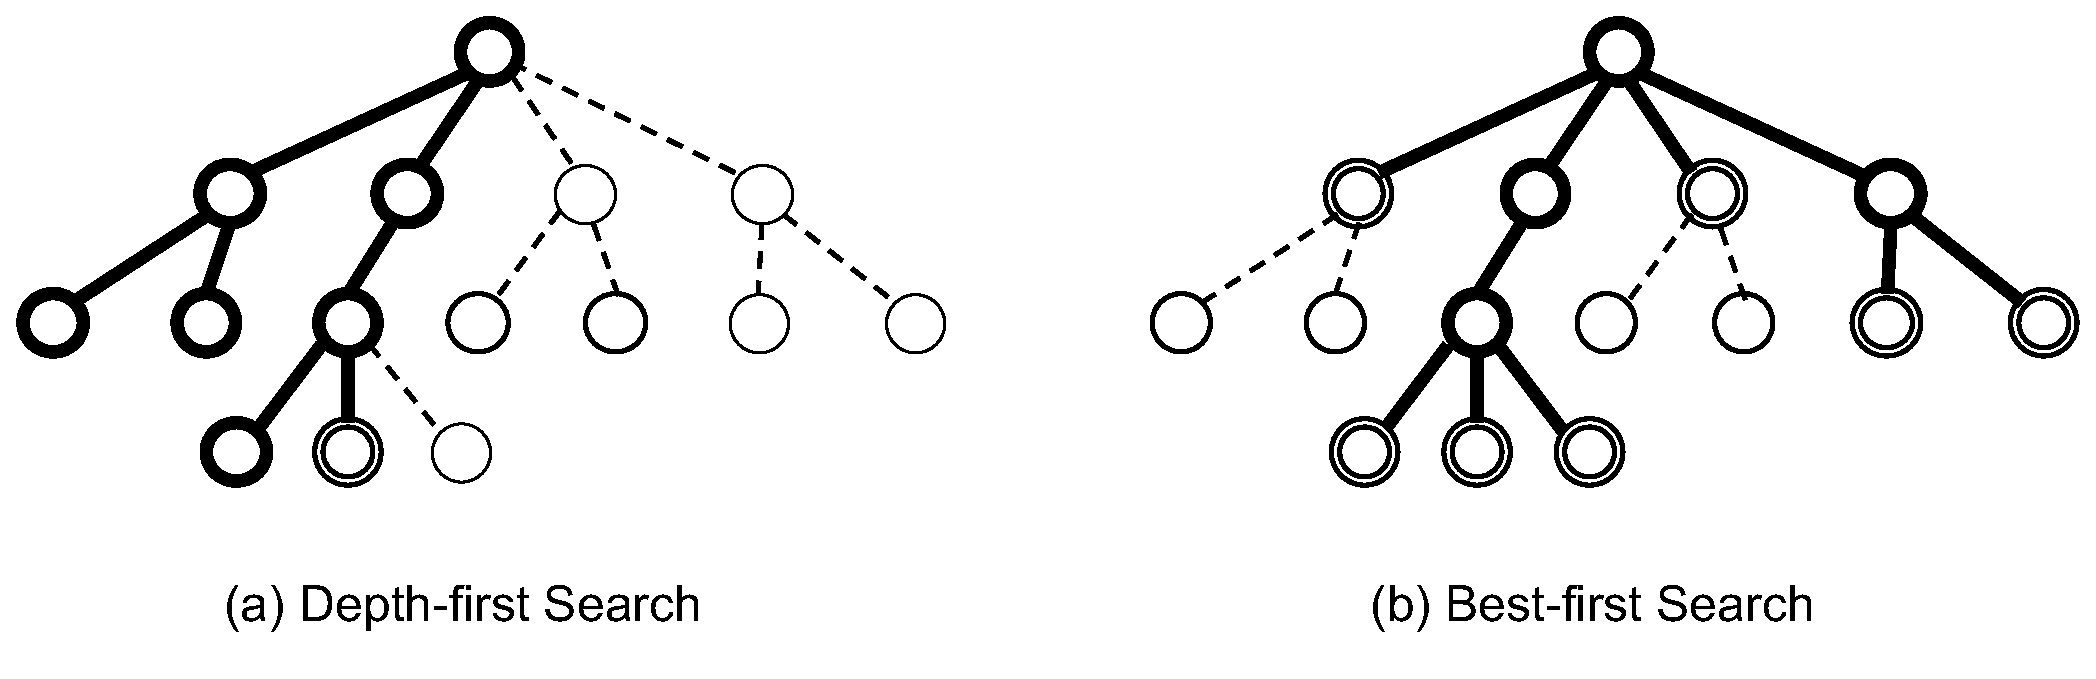
\includegraphics[width=0.9\linewidth]{img/search.eps}
	\caption{
		Depth-first vs. Best-first.
		The bold circles show already searched nodes and 
		double circles show the candidate nodes for next expansion}
  	\label{fig:search}
\end{figure}

\section{Proposed Method}
The previous method \cite{Shirakawa:2018} employs a naive depth-first search policy. 
This policy does not capture factors such as the nature of the dataset or the situation of current search.
The previous method calculate $DScore$ and its lower bound for every subgraph, 
so there is no additional cost for using these values in search policies.
In this section, using these values, 
we propose two efficient search policies 
based on $(i)$ Best-first Search and $(ii)$ Monte Carlo Tree Search.

\subsection{Best-first Search}
Best-first searching \cite{pearl:1984} is a search policy 
that expands from the best node based on some evaluation value, shown as Figure \ref{fig:search} (b).
The A* algorithm \cite{hart:1968} and Dijkstra algorithm \cite{dijkstra:1959} are representative.

The previous method designed the pruning rule 
by calculating the bound value in (\ref{eq:bound_R}). 
In the proposed method, this bound value is set as the search priority of each node, 
and is applied to the best-first search.
The pseudocode is shown in Algorithm.~\ref{alg:bfs}.
The search starts from the root node, 
and selects the node with the highest bound from the expansion candidate set.
The child nodes of the selected node are expanded, 
and the score is calculated and added to the expansion candidate set.
The above operation is repeated until pruning is possible for all expansion candidate set.\\

\begin{algorithm2e}[H]
  \caption{Subgraph Search by Best-first Search}
  \label{alg:bfs}
  \KwIn{Training data $\D = \{ (G_1,r_1), (G_2,r_2), \dots, (G_N,r_N) \} $}
  \KwOut{Best score subgraph $g^*$}
  \Fn{Best-first Search($\D$)}{
	$candidate \leftarrow \{root\}$
    \Repeat{all candidate can be pruned}{
		$g \leftarrow \argmax_{candidate\ c} bound(c)$ \;
		$candidate \leftarrow candidate / {g}$ \;
		\ForAll{child c of g}{
      		\If{DScore(c) is better than $score^*$}{
	  		  $score^*$ $\leftarrow$ $DScore(c)$ \;
	  		  $g^*$ $\leftarrow$ $c$  \;
      		}
			$candidate \leftarrow candidate \cup {c}$ \;
		}
		
    }
    \KwRet{$g^*$} \;
  }
\end{algorithm2e}

\subsection{Monte Carlo Tree Search}
We consider to apply Monte Carlo tree search (MCTS) 
\cite{Levente:2006, Romaric:2010, Cameron:2012} to our problem. 
MCTS is widely known as the method used in computer Go. 
It is also applied in various fields such as feature selection. 
One of them, Upper Confidence Bounds for Tree (UCT) algorithm 
\cite{Levente:2006} is empirically highly evaluated as a way to find good solutions within a limited budget.
This method resolves the exploration-exploitation problem using Upper Confidence Bound (UCB),
which allows to estimate the expected reward of each child.
The simplest UCB policy is called UCB1 and does not require the prior specific knowledge.
The policy selects to search child node $i$ that maximizes
\begin{equation}
  \label{eq:ucb}
  UCB1 = \bar{X}_{i} + C \times \sqrt{\frac{\ln{n}}{2 n_{i}}}
\end{equation}
where $\bar{X}_{i}$ is the average reward from child node $i$, 
$n_{i}$ is the number of times child node $i$ was selected, 
$n$ is the number of times parent node of $i$ was selected,
and $C$ is an exploration constant.
The left term encourages the exploitation of high expected reward child,
and the right term encourages the exploration of less visited child.

The UCT algorithm is an iterative method 
doing the four operations of selection, expansion, 
simulation, and backpropagation up to a predefined computational cost, shown as Figure \ref{fig:MCTS}.
\begin{figure}[t]
  \centering
  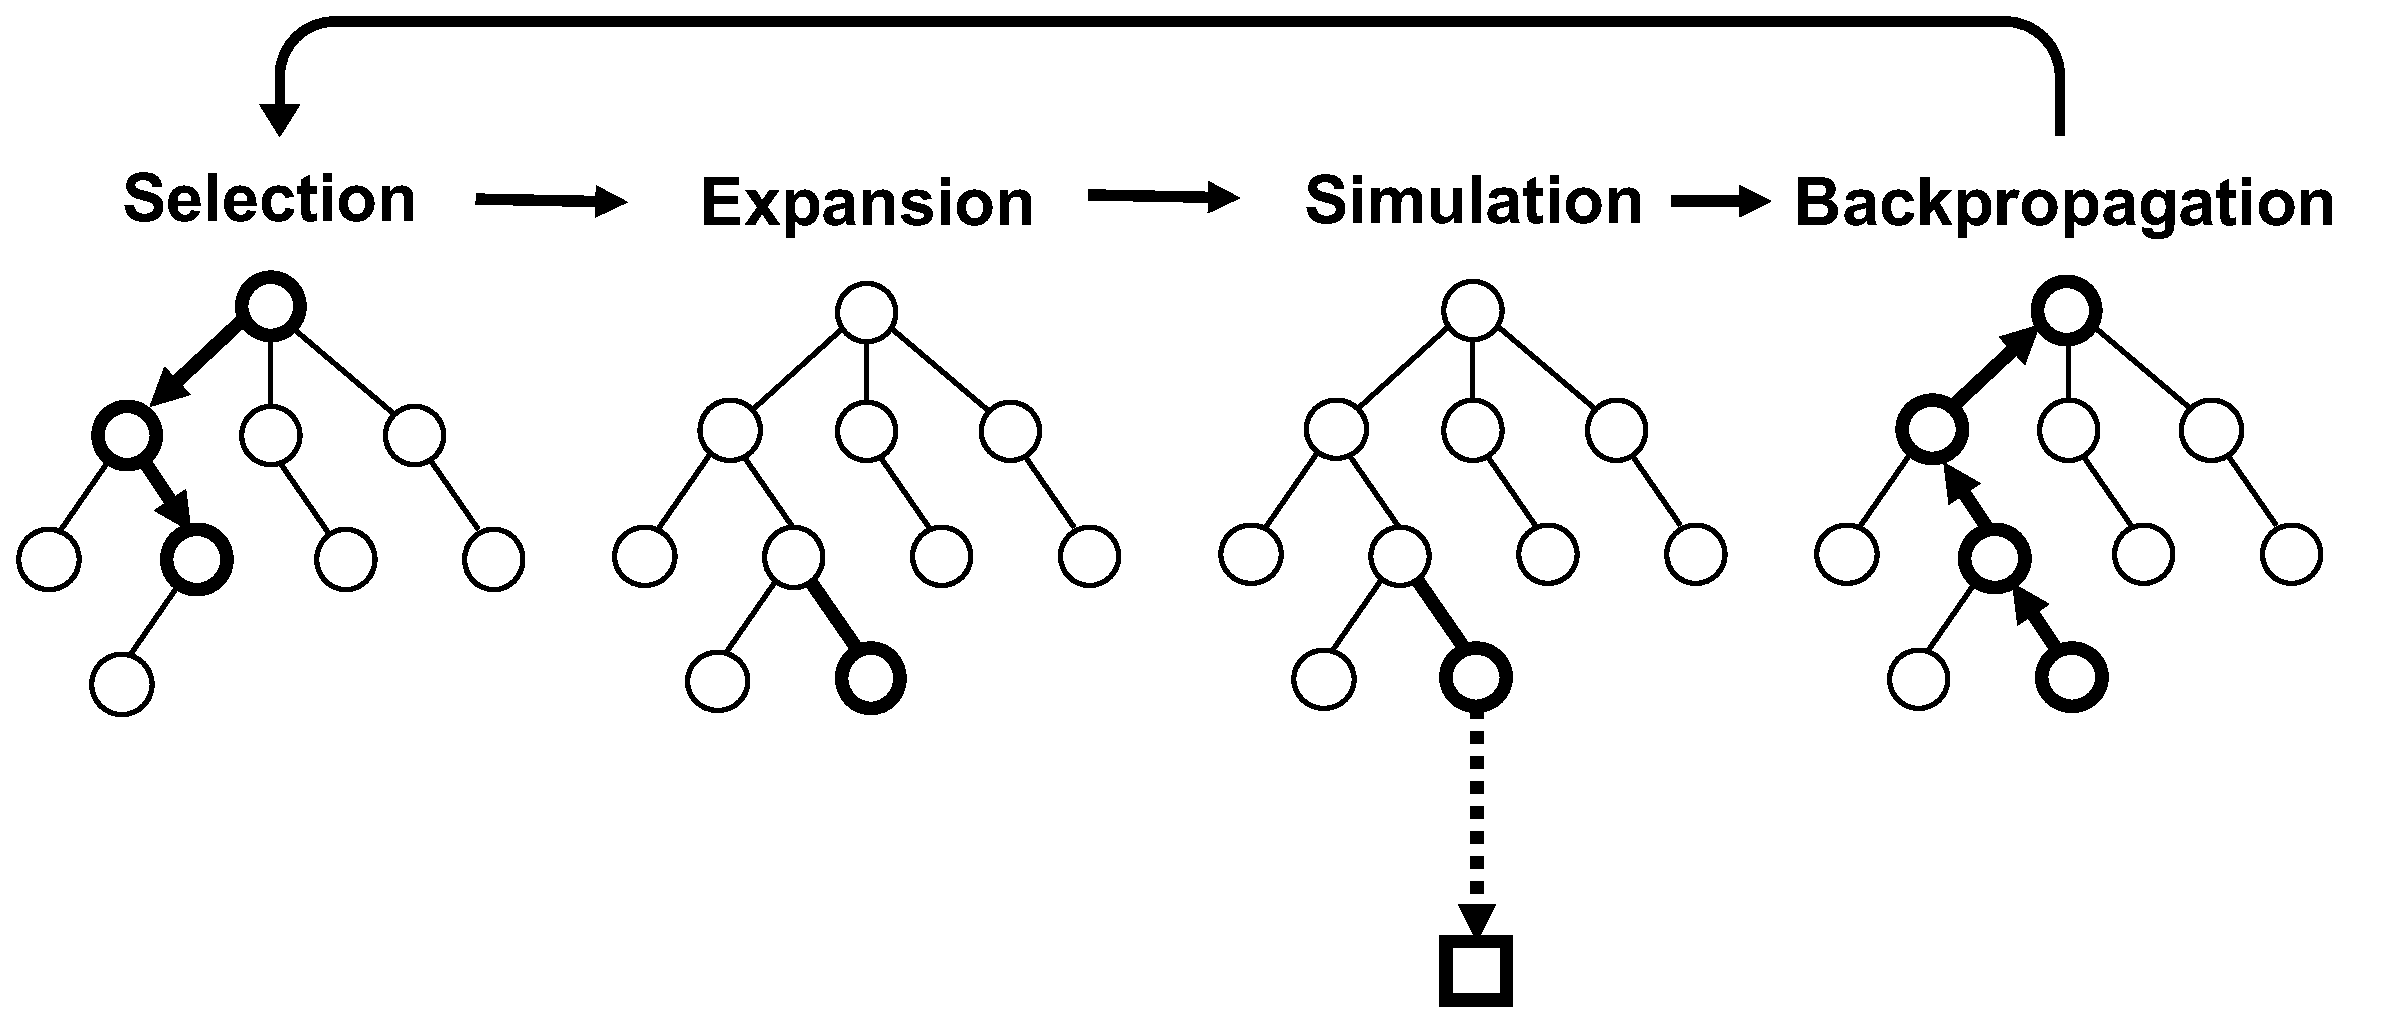
\includegraphics[width=0.9\linewidth]{img/MCTS.eps}
  \caption{One circle of processes in UCT}
  \label{fig:MCTS}
\end{figure}


\begin{enumerate}
	\item{Selection}:

	~~Start from the root node, and select the child node repeatedly 
	based on the value of $UCB1$ until the expandable node is reached.
	A node is expandable if it represents a non-terminal state and has unvisited children.

	\item{Expansion}:

	~~One random child node that is unvisited is expanded.
	In this operation, we consider the same pruning condition as (\ref{eq:bound_R}). 
	If the random select node can be pruned, another node is reselected and expanded.

	\item{Simulation}:
	
	~~A Monte Carlo simulation is run from the new expanded node,
	and repeatedly select a child randomly from the available children.
	This simulation stops if the simulation node has no children or 
	is based on a stochastic condition known as a stopping feature used in \cite{Romaric:2010}.
	The stochastic condition is $1 - q^{d}$ depending on the simulation node level d,
	where $q < 1$ is a parameter and $q = 1 - 10^{-1}$ in the present paper.
	
	\item{Backpropagation}:

	~~Calculate the reward of the node $g$ obtained by simulation.
	To align the range to $[0, 1]$, reward is defined, 
	\begin{eqnarray}
		reward(g) = -DScore(g) / \tss(\D)
	\end{eqnarray}
	this value will be large if discrimination is successful, otherwise small.
	Then backpropagate this reward to the nodes selected in selection and expansion phase.
\end{enumerate}

%TODO
\subsubsection*{UCT for Subgraph Feature Space}
In this problem setting, the search space is not given in advance.
Therefore, we need to construct a search space that matches the given dataset 
and subgraph search at the same time.
When Monte Carlo simulation is performed in this problem, 
it is necessary to enumerate all the child nodes for each simulation node, which requires a large cost.
We design a low-cost simulation method 
since the simulation cost has a big influence on the search efficiency.

First, a graph including simulation node is randomly selected from the dataset.
Expand the subgraph represented by the simulation node on the selected graph.
If an expanded subgraph is available(minimum order defined by \cite{Yan:2002}), 
this simulation is taken, otherwise it is repeated. \\

The entire procedure of the proposed algorithm is illustrated with pseudocode in 
Algorithm.~\ref{alg:uct}, \ref{alg:four_operations}.\\

\begin{algorithm2e}[H]
  \caption{Subgraph Search by UCT}
  \label{alg:uct}
  \KwIn{Training data $\D = \{ (G_1,r_1), (G_2,r_2), \dots, (G_N,r_N) \} $}
  \KwOut{Best score subgraph $g^*$}
  \Fn{UCT($\D$)}{
    \Repeat{predefined cost is exhausted}{
      \g $\leftarrow $ Selection(root) \;
      \g $\leftarrow $ Expansion(\g) \;
      \If{DScore(g) is better than $score^*$}{
		$score^*$ $\leftarrow$ $DScore(g)$ \;
		$g^*$ $\leftarrow$ \g  \;
      }
      $s \leftarrow $ Simulation(\g) \;
      Backpropagation($s, g$) \;
    }
    \KwRet{$g^*$} \;
  }
\end{algorithm2e}

\begin{algorithm2e}[H]
  \caption{Four Basic Operations in UCT}
  \label{alg:four_operations}
  \Fn{Selection($g$)}{
	\While{$g$ is expandable}{
		$g \leftarrow \argmax_{children\ c\ of\ g} \bar{X}_{c} + C \times \sqrt{\frac{\ln{n_{g}}}{2 n_{c}}}$ \;

	}
    \KwRet{$g$} \;
  }
  \Fn{Expansion($g$)}{
    \Repeat{g' is not pruned}{
	  $g' \leftarrow random(\{children\ c\ of\ g\})$ \;
	}
      \KwRet{$g'$} \;
  }
  \Fn{Simulation($g$)}{
	$s \leftarrow g$ \;
	\While{$s$ has some child and not enough stochastic condition}{
	  \Repeat{$s'$ is enough to minimum order}{
	  	$G \leftarrow random(\D)$ \;
	  	$s' \leftarrow random\ expansion\ from\ s\ on\ G$ \;
	  }
	  $s \leftarrow s'$ \;
	}
      \KwRet{$s$} \;
  }
  \Fn{Backpropagation($s, g$)}{
	$X = reward(s)$ \;
	\While{$g \neq NULL$}{
		$n_{g} \leftarrow n_{g} + 1$ \;
		$\bar{X}_{g} \leftarrow \frac{\bar{X}_{g} \times (n_{g} -1) + X}{n_{g}}$ \;
		$g \leftarrow parent\ of\ g$ \;
	}
  }
\end{algorithm2e}

\section{Experiments}
\subsection{Datasets}
We also evaluate the performance based on the most typical benchmark on real datasets:
the quantitative structure-activity relationship (QSAR). 
We select Four binary-classification datasets (CPDB, Mutag, AIDS(CAvsCM), CAS) in Table~\ref{tbl:dataset}: 
CPDB and Mutag for mutagenicity tests and AIDS(CAvsCM) for antiviral tests.
All chemical structures are encoded as molecular graphs using RDKit\footnote{\url{http://www.rdkit.org/}}, 
and some structures in the raw data are removed by chemical sanitization\footnote{
Due to this pre-processing, the number of datasets differs from that 
in the simple molecular graphs in the literature, 
where the nodes are labeled by atom type, and the edges are labeled by bond type.}.
We simply apply a node labeling by the RDKit default atom invariants (edges not labeled), i.e., 
atom type, \# of non-H neighbors, \# of Hs, charge, isotope, and inRing properties. 
These default atom invariants use connectivity information similar to that used for the well-known 
ECFP family of fingerprints\cite{Rogers:2010}. See \cite{Kearnes2016} for more elaborate encodings.

\tabcolsep = 6pt
\begin{table}[h]
  \centering
  \caption{Dataset summary}
  \label{tbl:dataset}
  	\begin{tabular}{lcccc}
		\thickhline
		Dataset			& CPDB           & Mutag        & AIDS(CAvsCM)     & CAS	\\  \hline
		\# data			& 684            & 188          & 1503             & 4337	\\
		\# ($y=+1,-1$)	& (341, 343)     & (125, 63)    & (422, 1081)      & (2401, 1936)	\\  
		\# nodes		& 25.2           & 26.3         & 59.0             & 30.3	\\  
		\# edges		& 25.6           & 28.1         & 61.6             & 31.3	\\  
		\thickhline
		\end{tabular}
  \leftline{\hspace*{2pt} \# of nodes and edges are average.}
\end{table}

\subsection{UNDER CONSTRUCTION}

\begin{comment}
\subsection{MCTS Cost Performance Comparison to Exact Search}
\label{sec:experimentspeed}
As previously mentioned in Section~\ref{sec:relatedwork}, \ref{sec:ourapproach}, 
%our method is based on \cite{Shirakawa:2018} that search optimal feature exactly using tricky pruning, 
our method is based on that search optimal feature exactly using tricky pruning, 
in this section we call the previous method GTB-exact, and proposed method GTB-MCTS.

MCTS is able to control the cost of feature search by setting the number of Monte Carlo simulations.
We investigate the cost performance of MCTS and compare with previous exact method.
Each hyperparameters is shared(the number of trees: 100, max tree depth: 3, stepsize: 1.0) 
and MCTS specific parameters is fixed(exploration constant: 1).
In this experimental setup, AIDS(CAvsCM) is used 
and the maximum subgraph size of feature search space is set to 10.
Since GTB-MCTS has randomness in the model, 10 model averages and variance values are used for evaluation.
Fig~\ref{fig:costperformance} shows the model construction time, training loss, and test accuracy compared
among each cost GTB-MCTS(the number of Monte Carlo simulations = [10,100,200,300,400,500]) and GTB-exact.
The left figure is log-scale, and this shows the construction time of GTB-MCTS increases linearly 
with the number of Monte Carlo simulations.
The lower the search cost, the greater the training loss mean,
however the test accuracy is higher than GTB-exact at lower search cost.
For example, the GTB-MCTS(the number of Monte Carlo simulations = 100) is build the higher accuracy model 
about 100 times faster than GTB-exact.
It is interesting that the accuracy can be improved in spite of reducing the search cost.
Then we investigate the detail of the features used in these models.

Fig~\ref{fig:featuresize} shows the size ratio of the features used to learn the model.
We can observe that the features that GTB-exact uses for learning are almost big, 
about 80\% are subgraphs with 9 or 10 edges.
On the other hand, GTB-MCTS has a balanced features size ratio unless the search cost is too low.
Therefore, GTB-MCTS has higher generalization ability than GTB-exact, which led to improve the test accuracy.
\begin{figure}[t]
 \centering
  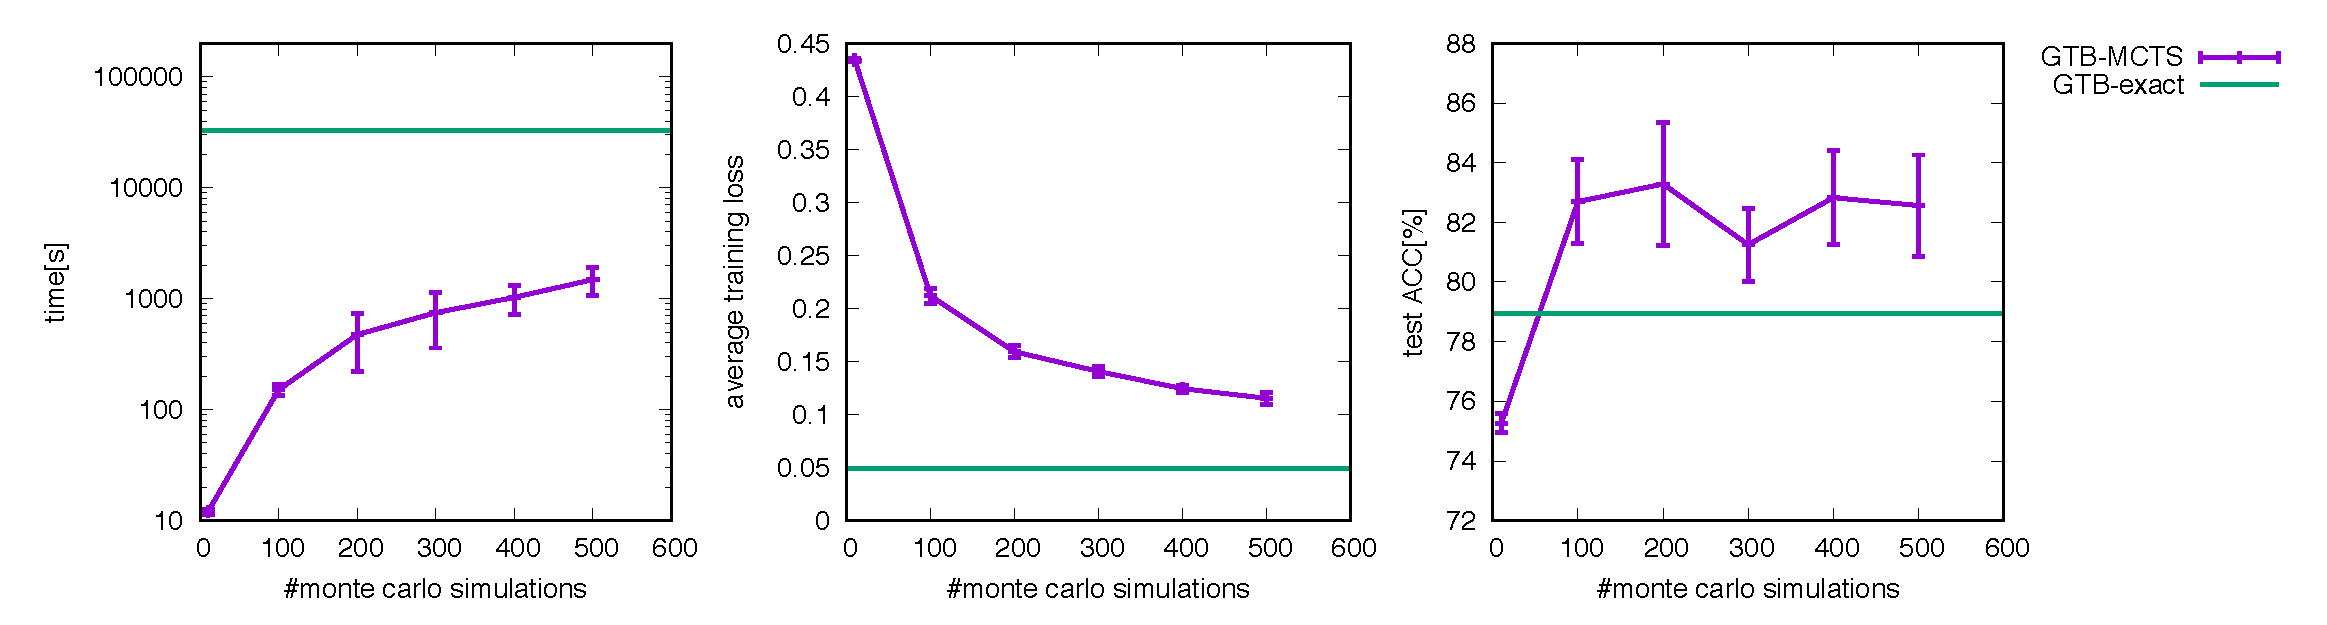
\includegraphics[width=1\textwidth]{img/speed.eps}
   \caption{Search cost performance}
   \label{fig:costperformance}
\end{figure}
\begin{figure}[t]
 \centering
  \includegraphics[width=0.55\textwidth]{img/feature_rate.eps}
   \caption{Features size ratio}
   \label{fig:featuresize}
\end{figure}

\subsection{Accuracy for the QSAR}
Tables~\ref{tbl:acc} shows the performance results obtained 
by 10-fold cross validations for QSAR datasets.
We use the same two nonlinear methods used before 
and one linear method, gBoost\cite{Saigo:2009} that is the basis of our method. 
The hyperparameter tuning is performed for the ranges described in Table~\ref{tbl:param}, 
and the best parameters are also listed in Table~\ref{tbl:bestParam}.
We can observe that nonlinear methods often outperform the linear method. 
At the same time, our proposed method GTB-MCTS achieves the best performance except for CPDB. 
The overall accuracy for the CPDB is also the second, 
this shows that our proposed method is able to be a good solution for real datasets.

\tabcolsep = 13pt
\begin{table}[t]
  \centering
  \caption{Hyperparameter settings for the QSAR}
  \label{tbl:param}
  \scalebox{0.85}{
   \begin{tabular}{llcl}
     \multicolumn{3}{l}{\textit{Common}} \\
     \thickhline
     %\multicolumn{2}{|l}{min support} & $m$(\%) & 10, 5, 2.5, 0 \\
     \multicolumn{2}{l}{max subgraph size (\# edges)} & $x$ & 4, 6, 8 \\
     \thickhline
     \multicolumn{3}{l}{} \\
     \multicolumn{3}{l}{\textit{Model specific}} \\
     \thickhline
     GTB- & max tree depth & $d$ & 1, 3, 5 \\
     (MCTS, exact) & stepsize & $\eta$ & 0.1, 0.4, 0.7, 1.0 \\
     ~ & \# trees & $k$ & 1-500 \\
     \hdashline[2pt/1pt]
     (MCTS) & \# monte carlo simulations & $i$ & 100, 300, 500 \\
     ~ & exploration constant & $c$ & 1, 10, 100 \\
     \hline
     gBoost & regularization & $\nu$ & {0.01, 0.1, 0.2, 0.3,}{0.4, 0.5, 0.6} \\
     \thickhline
   \end{tabular}
  }
\end{table}

\tabcolsep = 7pt
\begin{table*}[t]
  \centering
  \caption{Prediction accuracy (\%) for the QSAR}
  \label{tbl:acc}
  \scalebox{0.87}{
  	 \begin{tabular}{lcccccc}
  	   \thickhline
  	   ~								& CPDB						& ~							& Mutag						& ~							& AIDS(CAvsCM)						& ~ 						\\
  	   ~   							& ACC       				& AUC       				& ACC       				& AUC       				& ACC                 				& AUC              			\\ \hline
  	   \multicolumn{7}{l}{\textit{Nonlinear models}} \\
  	   \ss{GTB-MCTS}{~}                & \ss{79.0}{($\pm$2.7)}     & \ss{83.7}{($\pm$2.7)}     & \fss{91.0}{($\pm$5.0)}  	& \fss{94.8}{($\pm$5.0)}   	& \fss{84.4}{($\pm$2.8)}   			& \fss{85.3}{($\pm$2.8)}   	\\
  	   \ss{GTB-exact}{~}                		& \fss{80.3}{($\pm$4.5)}    & \ss{84.9}{($\pm$4.5)}    & \ss{89.4}{($\pm$6.0)}  	& \ss{94.2}{($\pm$6.0)}   	& \ss{84.0}{($\pm$1.7)}   			& \ss{82.5}{($\pm$1.7)}   	\\ \hline
  	   \multicolumn{7}{l}{\textit{Linear models}} \\
  	   \ss{gBoost}{~}                	& \ss{77.9}{($\pm$6.2)}     & \ss{81.7}{($\pm$5.8)}     & \ss{85.0}{($\pm$1.5)}  	& \fss{94.8}{($\pm$5.5)}   	& \ss{83.9}{($\pm$3.6)}   			& \ss{69.0}{($\pm$8.1)}   	\\ \hline
  	   \hline
  	   \multicolumn{7}{l}{\textit{Reported values in literature}} \\
  	   L1-LogReg \cite{takigawa:2017} 	& 78.3 						& -    						& -                      	& -  						& -					   				& -					   	\\
  	   MGK \cite{Saigo:2009}		 	& 76.5   					& 75.6 						& 80.8                     	& 90.1 						& 76.2				   				& 76.0					   	\\
  	   freqSVM \cite{Saigo:2009} 		& 77.8 						& 84.5 						& 80.8                     	& 90.6 						& 78.2					   			& 80.8					   	\\
  	   gBoost \cite{Saigo:2009}		 	& 78.8   				& \fst{85.4} 				& 85.2                     	& 92.6 						& 80.2				   				& 77.4					   	\\
  	   WL shortest path \cite{Shrvashidze:2011}	& -   						& -    						& 83.7                  	& -  						& -					   			& -					   	\\
  	   Random walk \cite{Shrvashidze:2011} 		& -   						& -    						& 80.7                    	& -  						& -					   			& -					   	\\
  	   Shortest path \cite{Shrvashidze:2011} 		& -   						& -    						& 87.2                     	& -  						& -					   			& -					   	\\
  	   \thickhline
  	 \end{tabular}
  }
\end{table*}

\tabcolsep = 6.5pt
\begin{table*}[t]
  \centering
  \caption{Best hyperparameters}
  \label{tbl:bestParam}
  	\scalebox{0.87}{
  	\begin{tabular}{lllll}
  	  \thickhline
  	  ~                    & CPDB               				& Mutag            					& AID(CAvsCM)               \\  \hline
  	  GTB-MCTS             & $x8~d1~\eta0.7~k23~i500~c10$ 	& $x8~d1~\eta0.4~k92~i500~c100$ 	& $x6~d3~\eta0.4~k349~i500~c1$  	\\  
  	  GTB-exact    		   & $x8~d1~\eta0.4~k497$ 			& $x6~d1~\eta0.4~k289$				& $x6~d5~\eta0.4~k8$ 	 	\\ 
  	  gBoost               & $x6~\nu0.3         $ 			& $x6~\nu0.4       $ 				& $x8~\nu0.4         $		\\  
  	  \thickhline
  	\end{tabular}
  }
\end{table*}
\end{comment}

\section{Conclusion}
In summary, we proposed an efficient approximate search method 
by applying the MCTS algorithm and the best-first search algorithm to the subgraph feature space.
These approximate search methods were able to obtain better solutions compared 
to existing naive search policy.
In addition, the learning model constructed by performing this search iteratively 
reduced the model construction cost from about 1/10 to 1/200 
while improving the accuracy compared to the existing exact search model.
This confirms that the approximate search leads to an improvement in the generalization performance, 
and may not only reduce the search cost but also provide a good solution for regularization.

However there are many challenges.
First, regarding cost constraint, 
there is no standard as to how much cost should be spent on a problem of what scale.
Currently, it is only experimentally determined, 
so it is easier to handle if the standard is set theoretically.
Second, the MCTS method used this paper is the most basic one. 
Considering more advanced methods and problem-specific heuristics will likely lead to better searches.

\begin{comment}
In summary, we proposed a novel efficient algorithm to learn the nonlinear model 
using subgraph indicators without any class constraint.
In addition to solving computational cost problems, 
our algorithm using MCTS improves generalization ability compared to previous methods.
The search efficiency and prediction accuracy were empirically evaluated by experiments using real datasets.

On the other hand, it is still necessary to investigate the proposed method. 
In this paper, we set the number of Monte Carlo simulations empirically, and there is no uniform standard.
Some MCTS methods may provide theoretical guarantees for searching.
Furthermore, the performance may be improved by adopting some advanced methods of MCTS 
and domain specific heuristics.
\end{comment}


%\bibliographystyle{prml}
\bibliographystyle{junsrt}
\bibliography{ref}

\small
\appendix
\input{appendix}

\end{document}
